\section{Introduction}
\label{intro}

\subsection{Current Status of Distributed Wind Nationally}
\label{intr_distr_wind}

Distributed wind generators can be defined as relatively small-scale turbines in the range of a few kilowatts [kW] to few megawatts [MW] that are interconnected to the power system at the distribution level, either as front-of-the-meter or behind-the-meter installations \cite{ackermann_distributed_2001}. From 2008 to 2018, distributed wind capacity in the United States has grown \hl{steadily} from 310 MW to 1,127 MW \cite{orrell_2018_2019}. Distributed wind installations are influenced both by resource availability and by policy initiatives and several states have dominated the distributed wind market in the past decade. For instance, Texas [191 MW], Iowa [187 MW], Minnesota [136 MW], Massachusetts [80 MW] and California [75 MW] account for approximately 60\% of cumulative installed capacities for distributed wind in the United States \cite{orrell_2018_2019}. 

\hl{break down distributed wind deployment by size categories!}

The distributed wind market, however, is completely overshadowed by utility-scale wind, which grew from 25, 065 MW to 96,433 MW in the same 2008 to 2018 time period \cite{wiser_2018_2019}. Distributed wind has also been surpassed by distributed solar PV, which grew from 582 MW\textsubscript{DC} in 2010 to 4,637 MW\textsubscript{DC} in 2018 \cite{solar_energy_industries_association_us_2019}. In 2018, distributed wind added only 50.5 MW of capacity while utility-scale wind added 7,588 MW and distributed solar PV added 4,637 MW\textsubscript{DC}. The cumulative capacity and annual capacity additions for distributed wind, utility-scale wind and distributed solar PV are shown in Figure ~\ref{fig:cumcaps}. % Although representing a significantly smaller share of distributed energy generating capacity relative to rooftop solar PV, the capacity of distributed wind has increased steadily in the United States over the past decade \cite{orrell_2018_2019}.\footnote{Total cumulative capacity for distributed rooftop PV in the United States by the end of 2018 was 4,871 MW\textsubscript{DC}, compared to 1,127 MW\textsubscript{AC} for distributed wind \cite{orrell_2018_2019, solar_energy_industries_association_us_2019}.}


\begin{conditionalfigure}[!htb]
  \centering
 	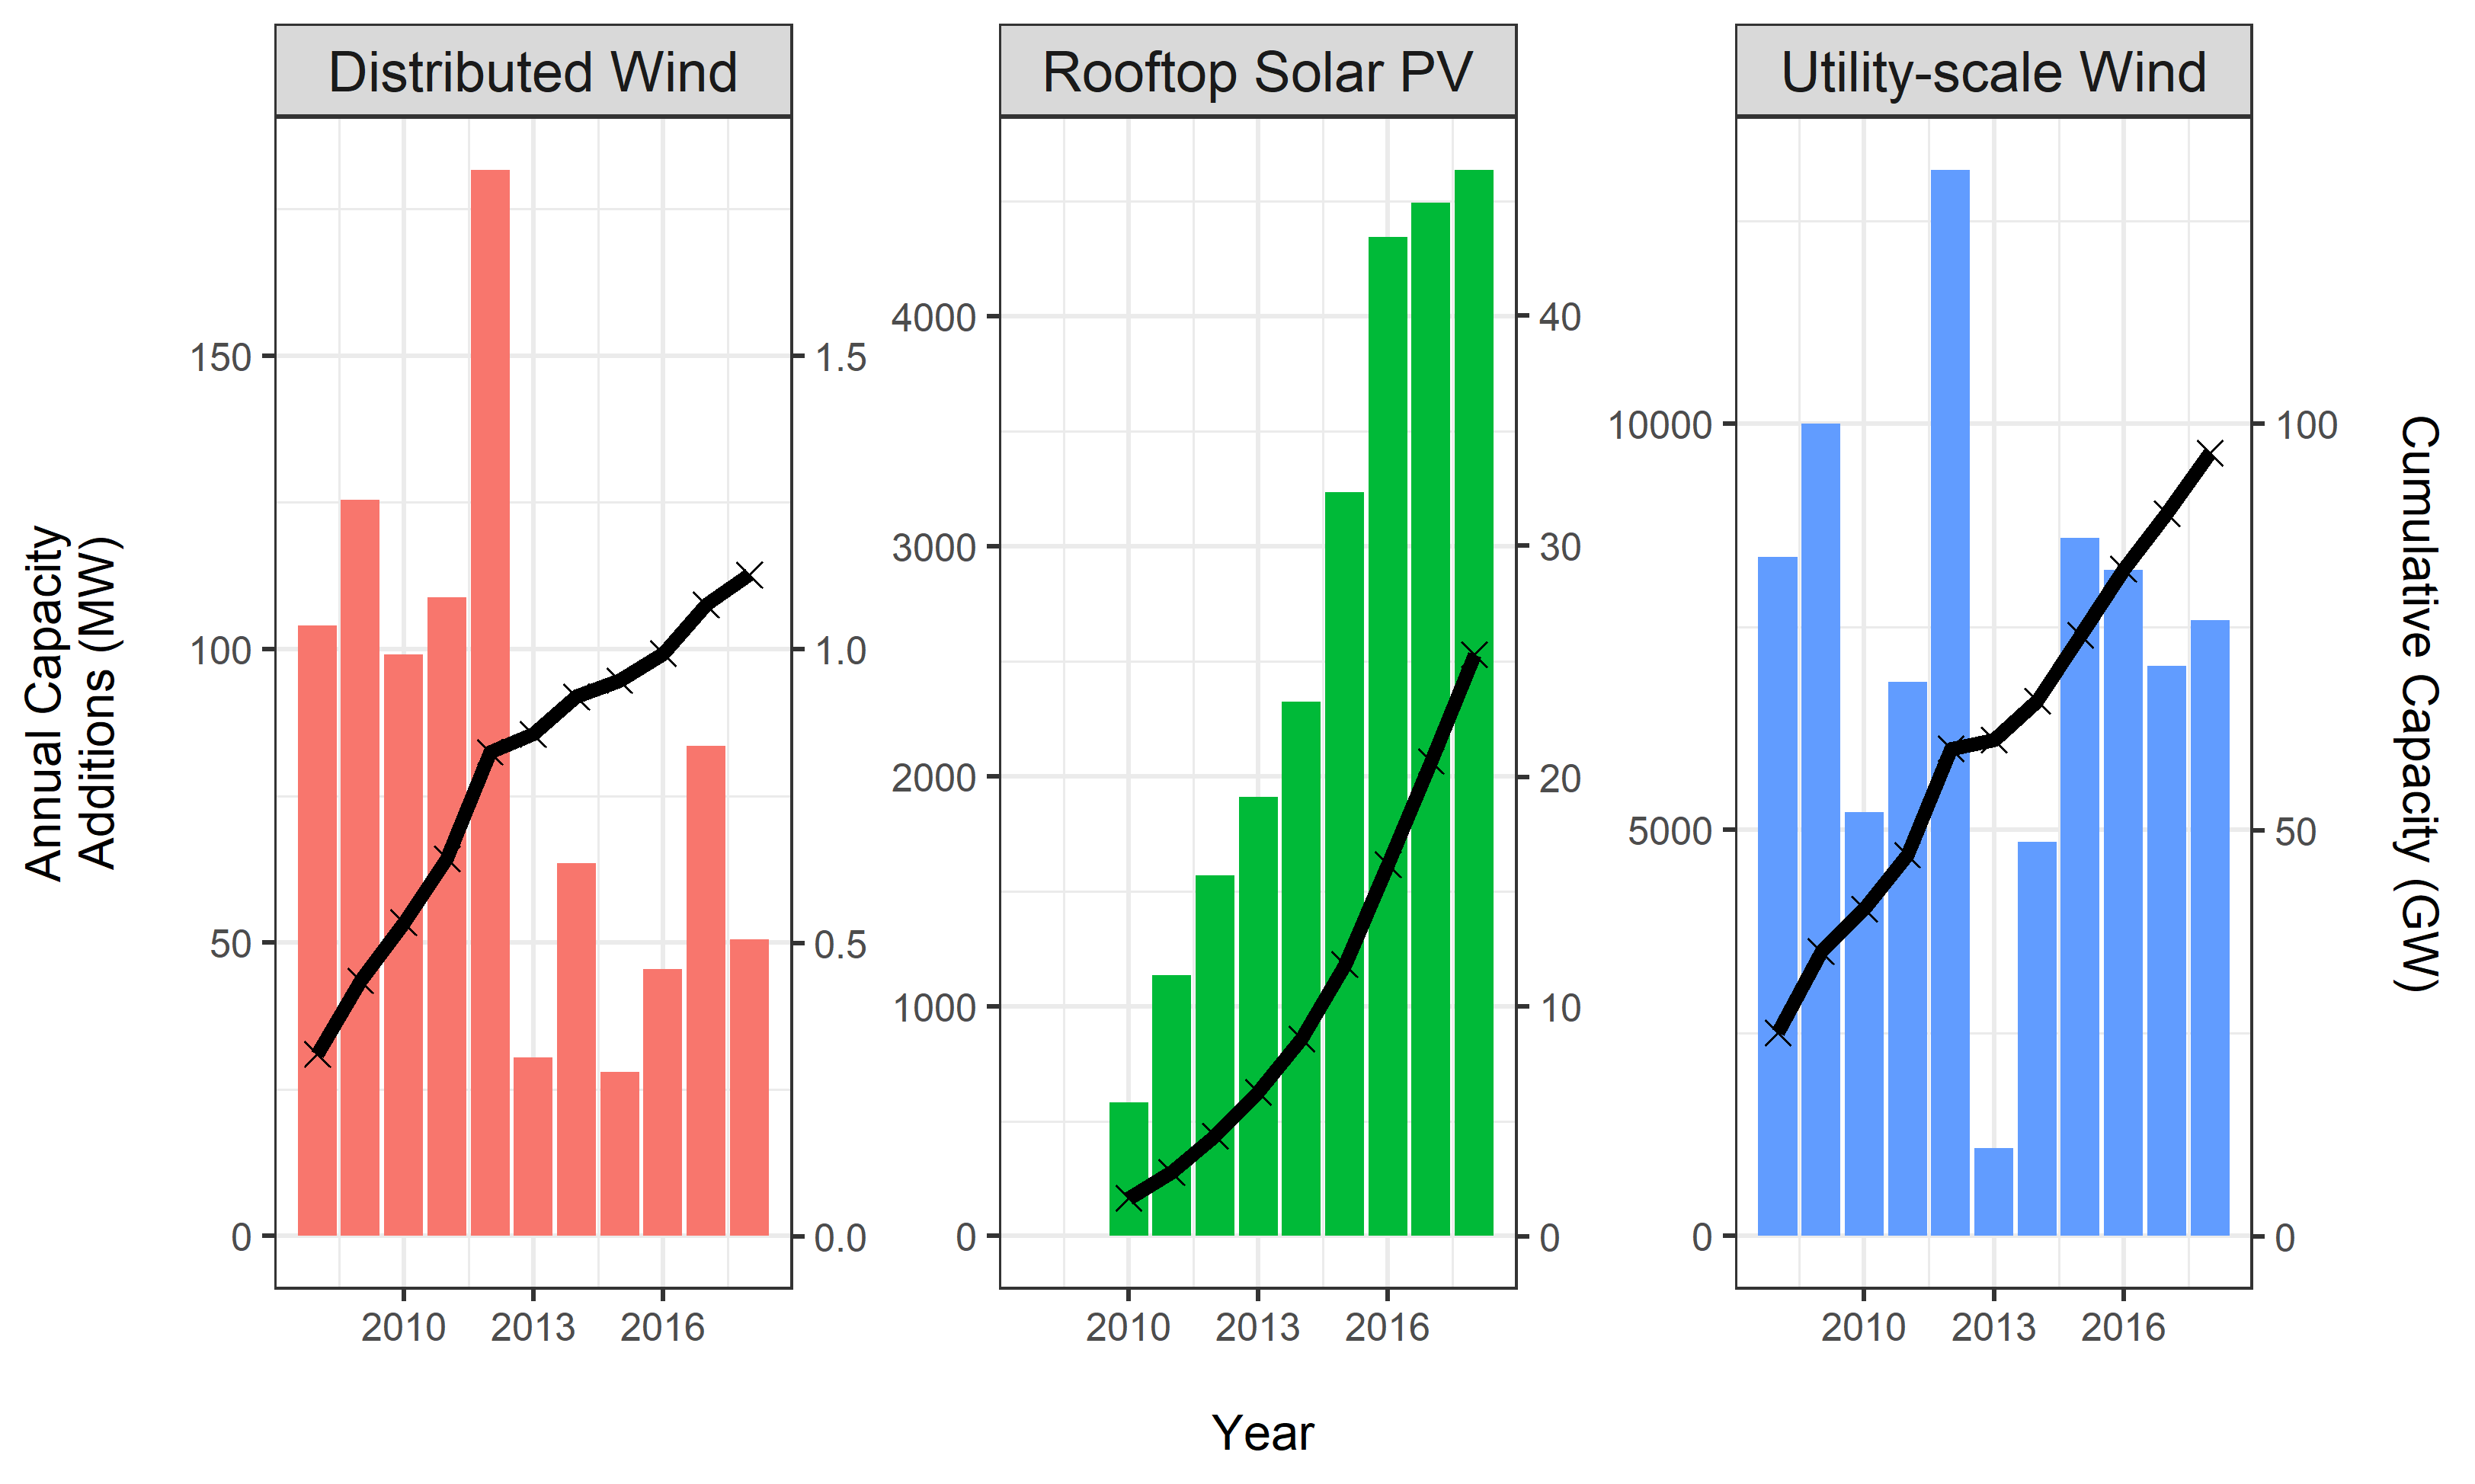
\includegraphics[width=\linewidth]{cumulative_us_capacities.png}
	\caption{Cumulative Capacity and Annual Capacity Additions of Distributed Wind, Distributed Solar PV and Utility-Scale Wind in the United States, 2008-2018}
	\label{fig:cumcaps}
\end{conditionalfigure}

The wide disparity in capacity growth between distributed wind and both utility-scale wind and distributed solar PV has generated interest in evaluating the technical and economic potential for the distributed wind industry. Technical potential is defined here as the achievable electricity generation capacity (MW) of a technology given information about an area's geographic or technology-specific constraints. Technical potential reflects the fact that not all physically available resources are developable, due to constraints to siting generation systems in particular areas (such as overhead canopy, obstruction of buildings, etc.) \cite{lee_exploring_2019}. Economic potential is defined here as a subset of the technical potential for economically viable generating capacity. Economic potential quantifies the generating capacity of systems capable of earning a positive net present value at a given point in time and reflects that fact that not all sytems which can technically be built will earn enough over their lifetime to offset the initial capital costs or recurring fuel and operation and maintenance costs associated with their generation \cite{mccabe_assessment_2018}. Figure ~\ref{fig:techeconpot} shows the connection between underlying physical resources and technical and economic potential.

\begin{conditionalfigure}[!htb]
  \centering
	  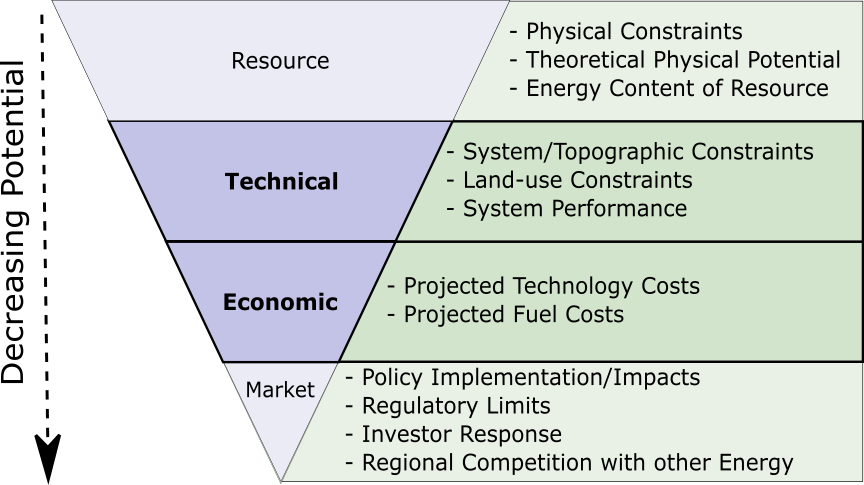
\includegraphics[width=.9\linewidth]{technical_economic_potential.png}
	  \caption{Framework Assessing Renewable Energy Potential and Associated Considerations. Adapted from \cite{lopez_us_2012}}
	  \label{fig:techeconpot}
\end{conditionalfigure}

Previous research has sought to evaluate the potential of distributed wind within select geographic regions, such as \citet*{mccabe_assessment_2018} which analyzed the economic potential for distributed wind in Colorado, Minnesota and New York. \citet*{ramdas_california_2019} likewise evaluated how the economic potential for distributed wind in California would be impacted by planned changes to the retail tariff as customers were shifted to time-of-use rates. \textcolor{pink}{\textsc{more studies on distributed wind capacity}}. This paper seeks to evaluate the technical and economic potential for distributed wind in the state of New York relative to utility-scale wind and distributed PV. In 2018 New York added 200 kW of distributed wind, bringing the state's cumulative capacity to 13.2 MW, compared to 1,987 MW of cumulative utility-scale wind and 434.3 MW\textsubscript{DC} of distributed solar PV \cite{orrell_2018_2019,wiser_2018_2019,solar_energy_industries_association_us_2019}. The state was chosen as it was an established (if not leading) distributed wind market with promising resource potential and welcoming policy environment.\footnote{Although currently expired, the Small Wind Incentive Program, administered by the New York State Energy Research and Development Authority (NYSERDA), offered up to 50\% rebates of the total installed costs for distributed wind generators (up to 2 MW in capacity) from 2016 to 2018 \cite{nyserda_public_2019}.} 

\hl{In addition to favorable resources, New York has a highly granular compensation mechanism to reward exports of energy from distributed resources depending on the time and location of the export.}

\subsection{Diffusion of New Technologies and its Relation to Distributed Wind}
\label{intro_diff}

% for the below have to keep in mind the fact that FOM distributed wind generation may be targeted by utilities after specific analysis
The diffusion of new distributed generation technologies is characterized by adoption among small pockets of the general public. For these customers, due to unique characteristics such as specific demand patterns, unique tariffs, higher than average utility bills, access to unique policy support, or personal opinions on clean generation, the costs associated with the distributed generation resource are outweighed by the economic and non-economic benefits of the technology before the general public. As these initial customers begin adopting the technology, it helps establish the market, which grows according to an ``S-curve'' as more and more customers begin consider the technology given its new visibility and lower prices (see Figure ~\ref{fig:bassscurve}) \textcolor{pink}{\textsc{source}}. While Bass diffusion models can adequately explain the adoption of distributed assets from a customer perspective, front-of-the-meter (FOM) distributed assets can be driven by slightly different processes \textcolor{red}{\textsc{source}}. 

\begin{conditionalfigure}[!htb]
  \centering
	  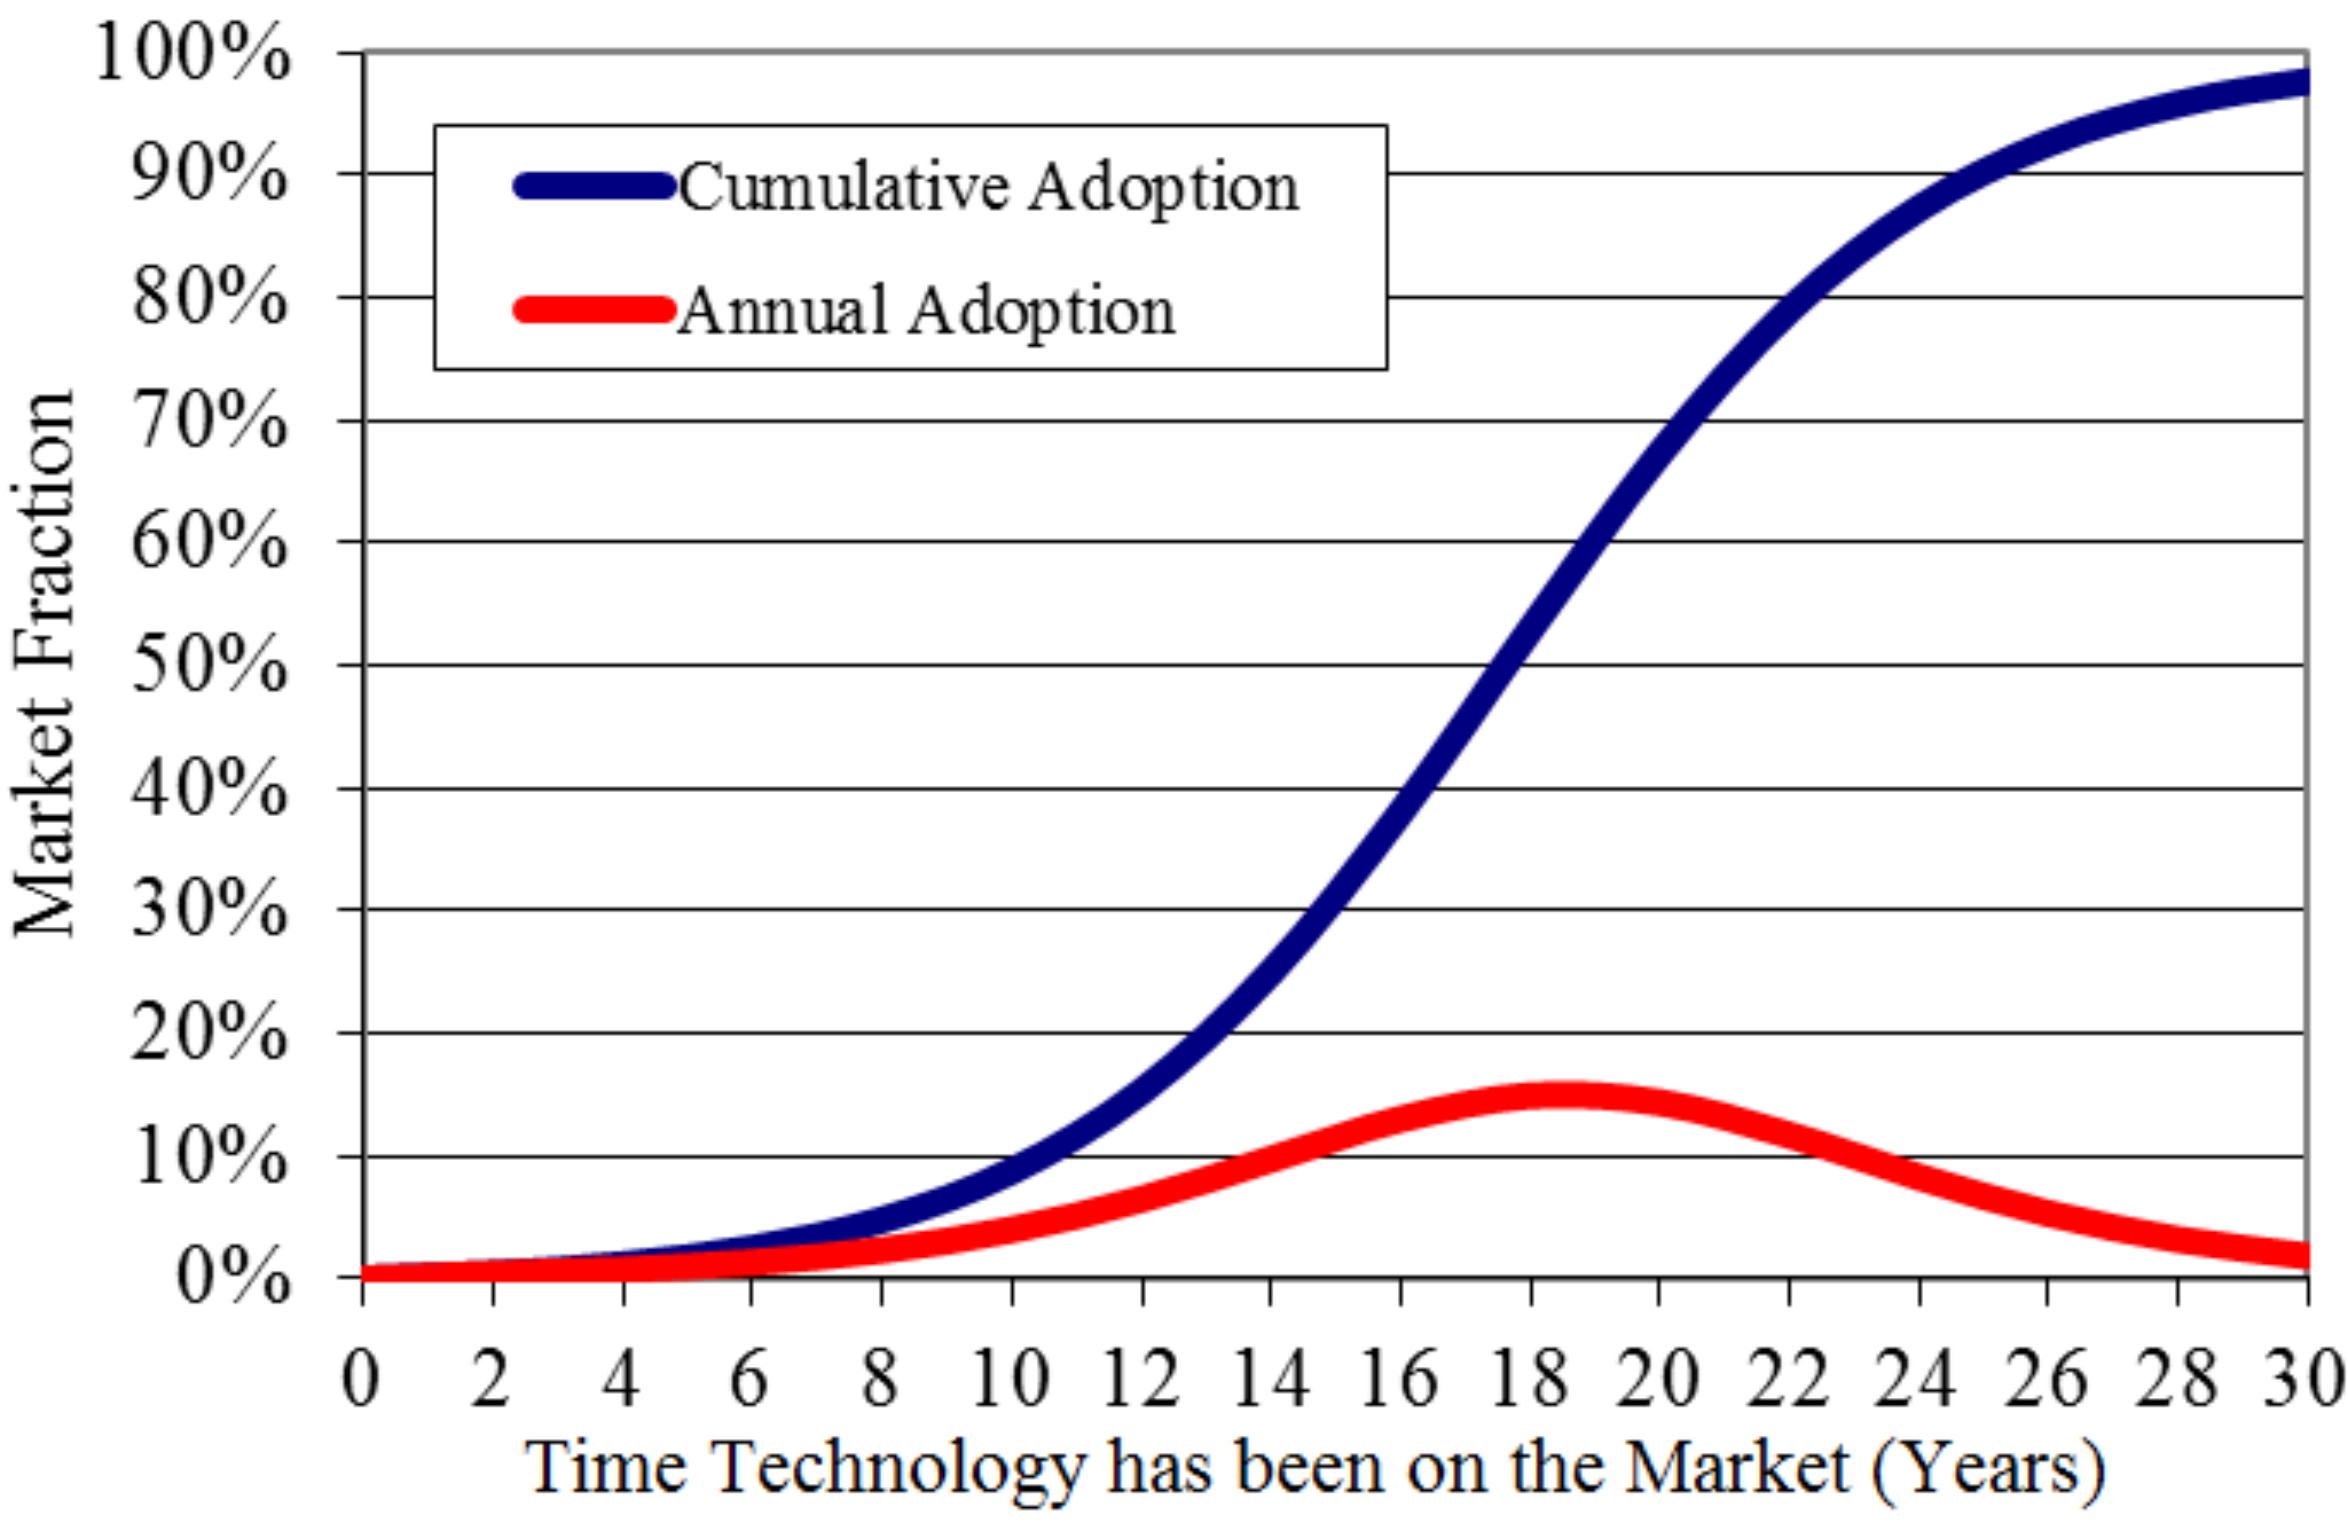
\includegraphics[width=.6\linewidth]{bass_diffusion_S-curve.png}
	  \caption{Annual and cumulative adoption rates simulated using the diffusion of innovations framework. Source: \citet{sigrin_distributed_2016}}
	  \label{fig:bassscurve}
\end{conditionalfigure}

For FOM assets, utilities may evaluate the ability of the resource to provide a unique set of services inaccessible to utility-scale assets, due to factors such as transmission constraints \textcolor{red}{\textsc{source}}. However, even though the adoption of these resources is not driven by individual customer decisions, the diffusion model can still accurately describe the trajectory of adoption as deployments are initially constrained to a small portion of the power system with the most advantageous conditions, but later expands to other parts of the grid as technology costs come down, driven partly by initial diffusions establishing a market \textsc{this whole paragraph is suspect and needs to be thoroughly reviewed and rewritten}. Whether customer-driven behind-the-meter deployments or utility-driven front-of-the-meter deployments, initial markets can be constrained to a small number of locations/applications/conditions. Identifying these limited locations/applications/conditions can help customers and utilities invest in economic deployments as well as help policymakers \hl{kickstart} local markets through targeted incentives or other measures. 

This identification, however, requires a sufficiently granular analysis as averages, whether of wind resources, tariff structures, siting availability or otherwise, can hide pockets in which conditions are sufficient to warrant investment in a given technology. Furthermore, in analyzing the potential adoption of a front-of-the-meter system by a utility, there must be a way to accurately monetize the many potential benefits such a system could accrue to the power system and utility as these economics are what is ultimately compared to technology costs when deciding whether or not to adopt. The 'Value of Distributed Generation' framework provides a useful methodology of quantifying the benefits of a distributed resource's exports that accrue to the the power system \cite{denholm_methods_2014}.

\subsection{The Value of Distributed Energy Resources}
\label{intro_vder}

In the aftermath of Hurricane Sandy, the New York Public Service Comission (NYPSC) proposed the Reforming the Energy Vision (REV), a fundamental overhaul of the regulatory and market structures surrounding the distribution system to address issues as diverse as concerns over carbon emissions, aging infrastructure and growing physical and cyber threats to the power system \cite{nypsc_reforming_2014}. As part of the REV initiative, NYPSC developed a new mechanism to compensate exports from distributed energy resources such as rooftop PV and distributed wind generators. The mechanism, called the Value of Distributed Energy Resources (VDER) is intended to ultimately replace the current compensation mechanism of net energy metering (NEM) \cite{nypsc_order_2017}. 

Under net energy metering, a customer is only billed for their net energy consumption (i.e. what the customer consumes less their exports to the grid), essentially rewarding a customer's exports at the retail rate of electricty \cite{zinaman_grid-connected_2017}. Net energy metering is a widely adopted compensation mechanism for distributed generation in the United States \cite{proudlove_50_2020}. Net energy metering, depending on the underlying retail tariff, is a farily invariant compensation mechanism that rewards exports to the grid at a flat rate regardless of the time of the injection of energy or of the underlying local grid conditions where the power is injected. Thus, NEM does not attempt to reward exports according to their value to the power system and concerns have been raised that this lack of accurate price signals can lead to cross-subsidization \textcolor{red}{\textsc{source}}. Furthermore, without adequate price signals, neither the deployment nor operation of these distributed generators can be aligned with power system needs, as customers, who tyically operate their systems to minimize their electricity bills, have little incentive or information to adjust their behavior \textcolor{red}{\textsc{source}}.

In response to these concerns, and in response to higher penetrations of distributed generation, many stakeholders have begun reevaluating how distributed generation should be compensated \cite{proudlove_50_2020}. One alternative compensation mechanism that has emerged is a Value of Distributed Generation framework, which attempts to quantify the value of an injection of distributed generation to the power system (or other stakeholders), often in high temporal and geosptial granularity \cite{denholm_methods_2014}. \hl{The values expressed/explored/rewarded under these frameworks vary from jurisdiction to jurisdiction, depending on their relative importance, as do the methods pursued to quantify the magnitude of the values.} Some common values explored include: 1) Energy; 2) Environmental; 3) Transmission and distribution losses; 4) Generating capacity; 5) Transmission and Distribution capacity \cite{proudlove_50_2020}.

The energy benefits associated with distributed generation represent the ability of the distributed system to offset generation from more expensive variable cost generators on the margin,\footnote{\hl{on the margin means ...}} which reduce their output in response to the distributed generation. The environmental benefits are closely related to the energy value, and \hl{typically} represent the reduced environmental costs (e.g., pollution) associated with the generators on the margin who reduce their output. Distributed generation can help avoid transmission and distribution losses as it is typically sited closer to load than \hl{utility-scale} generation (\textcolor{red}{\textsc{enough??}}. The generating capacity benefits of distributed generation represent the ability of distributed generation to help meet peak demand, \hl{which can reduce the amount of additional utility-scale generating capacity which must be procured to meet growth in peak demand.} Similarly, distributed generation can help reduce congestion on portions of the power system or reduce the need for additional transmission capacity by meeting demand locally \cite{denholm_methods_2014}.

%\subsection{Focus of This Research}
%\label{intro_thispaper}